%%----------------------------------------------------------------------------------------
%	PACKAGES AND THEMES
%----------------------------------------------------------------------------------------
\PassOptionsToPackage{table}{xcolor}
\documentclass[aspectratio=169,xcolor=dvipsnames,svgnames,x11names,fleqn]{beamer}
% \documentclass[aspectratio=169,xcolor=dvipsnames,fleqn]{beamer}

\usetheme{RedVelvet}

\usefonttheme[onlymath]{serif}
\newcommand{\showanswers}{yes}


\usepackage{xspace}
\usepackage{amsmath}
\usepackage{amssymb}
\usepackage{amsfonts}
\usepackage{color}
\usepackage{physics}
% \usepackage{mathbb}
\usepackage{rahul_math}
\usepackage{bigints}

\usepackage{graphicx} % Allows including images
\usepackage{booktabs} % Allows the use of \toprule, \midrule and \bottomrule in tables
\usepackage{tikz,pgfplots}

\usepackage{subfigure}
\usetikzlibrary{arrows}
\usepackage{minted}
\definecolor{LightGray}{gray}{0.9}
\definecolor{cream}{rgb}{0.92, 0.9, 0.55}
\definecolor{lightblue}{rgb}{0.68, 0.85, 0.9}


\usepackage{xcolor-material}
\usetikzlibrary{fit}
\usetikzlibrary{matrix}
\tikzset{%
apple/.pic={
    \fill [MaterialBrown] (-1/8,0)  arc (180:120:1 and 3/2) coordinate [pos=3/5] (@)-- ++(1/6,-1/7)  arc (120:180:5/4 and 3/2) -- cycle;
    \fill [MaterialLightGreen500] (0,-9/10)  .. controls ++(180:1/8) and ++(  0:1/4) .. (-1/3,  -1) .. controls ++(180:1/3) and ++(270:1/2) .. (  -1,   0) .. controls ++( 90:1/3) and ++(180:1/3) .. (-1/2, 3/4) .. controls ++(  0:1/8) and ++(135:1/8) .. (   0, 4/7)
    }
    }

\newcommand{\leftdoublequote}{\textcolor{blue}{\scalebox{3}{``}}}

\newcommand{\rightdoublequote}{\textcolor{blue}{\scalebox{3}{''}}}


\usepackage{textcomp}
\usepackage{fontawesome}
\usepackage{tikz,pgfplots}
\usetikzlibrary{shapes.callouts}
\usetikzlibrary{arrows}
\usetikzlibrary{shapes.geometric, positioning}
\pgfplotsset{compat=1.8} % or newest version

\usetikzlibrary{positioning}


\usepackage{bm}
\usepackage{relsize}



\tikzset{basic/.style={draw,fill=MediumBlue!20,text width=1em,text badly centered}}
\tikzset{input/.style={basic,circle}}
\tikzset{weights/.style={basic,rectangle}}
\tikzset{functions/.style={basic,circle,fill=MediumBlue!10}}



\usepackage{listofitems} % for \readlist to create arrays
\tikzstyle{mynode}=[thick,draw=MediumBlue,fill=MediumBlue!20,circle,minimum size=22]


\usepackage{overpic}

%----------------------------------------------------------------------------------------
%	TITLE PAGE
%----------------------------------------------------------------------------------------

\usepackage{tikz-qtree,tikz-qtree-compat}
\usetikzlibrary{tikzmark}
\usetikzlibrary{calc}

\usetikzlibrary{fit}
\tikzset{%
apple/.pic={
    \fill [MaterialBrown] (-1/8,0)  arc (180:120:1 and 3/2) coordinate [pos=3/5] (@)-- ++(1/6,-1/7)  arc (120:180:5/4 and 3/2) -- cycle;
    \fill [MaterialLightGreen500] (0,-9/10)  .. controls ++(180:1/8) and ++(  0:1/4) .. (-1/3,  -1) .. controls ++(180:1/3) and ++(270:1/2) .. (  -1,   0) .. controls ++( 90:1/3) and ++(180:1/3) .. (-1/2, 3/4) .. controls ++(  0:1/8) and ++(135:1/8) .. (   0, 4/7)
}
}
\usepackage{tikz-qtree,tikz-qtree-compat}
\usetikzlibrary{tikzmark}
\usetikzlibrary{calc}

\usetikzlibrary{positioning}


\usepackage{bm}
\usepackage{relsize}



\tikzset{basic/.style={draw,fill=MediumBlue!20,text width=1em,text badly centered}}
\tikzset{input/.style={basic,circle}}
\tikzset{weights/.style={basic,rectangle}}
\tikzset{functions/.style={basic,circle,fill=MediumBlue!10}}



\usepackage{listofitems} % for \readlist to create arrays
\tikzstyle{mynode}=[thick,draw=MediumBlue,fill=MediumBlue!20,circle,minimum size=22]


\newmdenv[
backgroundcolor=androidYellowLight,
linecolor=androidYellow,
linewidth=0.5pt,
roundcorner=10pt,
skipabove=\baselineskip,
skipbelow=\baselineskip
]{MintedFrame}

% Set minted options
\setminted{
fontsize=\footnotesize,
breaklines=true,
autogobble,
linenos,
frame=none
}


\title[CPE 487/587: Deep Learning]{CPE 486/586: Deep Learning for Engineering Applications} % The short title appears at the bottom of every slide, the full title is only on the title page
\subtitle{03 Introducing Deep Learning: Neural Networks}

\author[Rahul Bhadani] {{\Large \textbf{Rahul Bhadani}}}

\institute[UAH] % Your institution as it will appear on the bottom of every slide, maybe shorthand to save space
{
    Electrical \& Computer Engineering,  The University of Alabama in Huntsville
}
\date

% \titlegraphic{
%    \includegraphics[width=0.4\linewidth]{figures/UAH_primary.png}
% }

\begin{document}

%-------------------------------------------------
\begin{frame}
    \titlepage
\end{frame}

%-------------------------------------------------
\begin{frame}{Outline}
    \backgroundtableofcontents
\end{frame}


\section{A Single Perceptron: Build Blocks of Neural Network}

\begin{frame}
    \sectionpage
\end{frame}




%------------------------------------------------
\begin{frame}{A Neural Network}

\begin{center}
    
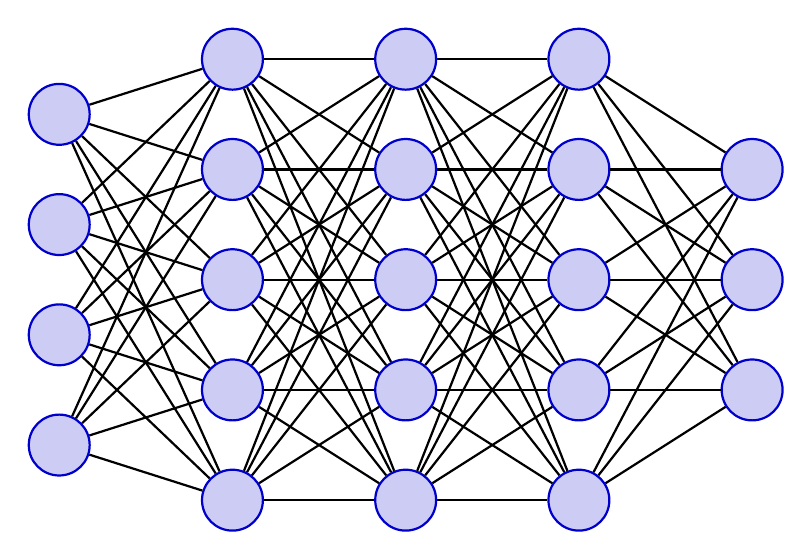
\begin{tikzpicture}[x=2.2cm,y=1.4cm]
  \readlist\Nnod{4,5,5,5,3} % number of nodes per layer
  % \Nnodlen = length of \Nnod (i.e. total number of layers)
  % \Nnod[1] = element (number of nodes) at index 1
  \foreachitem \N \in \Nnod{ % loop over layers
    % \N     = current element in this iteration (i.e. number of nodes for this layer)
    % \Ncnt  = index of current layer in this iteration
    \foreach \i [evaluate={\x=\Ncnt; \y=\N/2-\i+0.5; \prev=int(\Ncnt-1);}] in {1,...,\N}{ % loop over nodes
      \node[mynode] (N\Ncnt-\i) at (\x,\y) {};
      \ifnum\Ncnt>1 % connect to previous layer
        \foreach \j in {1,...,\Nnod[\prev]}{ % loop over nodes in previous layer
          \draw[thick] (N\prev-\j) -- (N\Ncnt-\i); % connect arrows directly
        }
      \fi % else: nothing to connect first layer
    }
  }
\end{tikzpicture}
\end{center}

\end{frame}


\begin{frame}{Linear Model}


\begin{gradblock}{}
    {
    \Huge
    \begin{align*}
    y = wx + b
    \end{align*}
    }
    \end{gradblock}
    
    For $n$ features, and introducing unit feature $x_0 = 1$ to incorporate $b$ into summation as $w_0$
    
    $$
    y = \sum_{i=0}^n w_i x_i
    $$
    
   or
   
   $$
   y = \wbf^\top \xbf
   $$

\end{frame}

\begin{frame}{Perceptron}

\begin{columns}
%------------------------------------------------
\column{.45\textwidth}

A neuron with unit-step for decision making:

\includegraphics[scale=0.55]{figures/Perceptron.pdf}

No hidden layer present.

Unit step is heaviside function \begin{align*}
g(z) = \begin{cases}
1, \quad \text{~~if~~} z \geq \theta\\
0, \quad \text{otherwise}
\end{cases}
\end{align*}

\LARGE

So what could be the problem here?

\column{.45\textwidth}
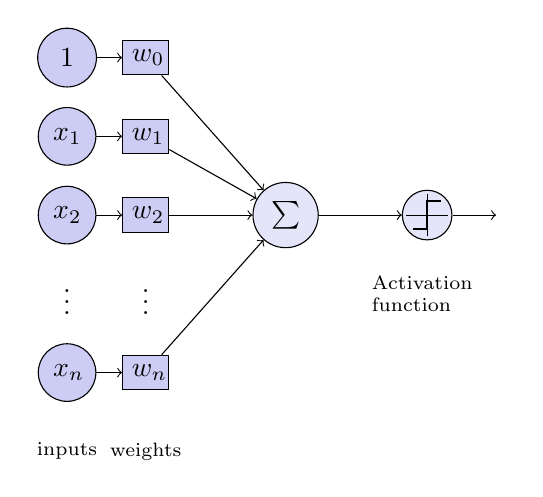
\begin{tikzpicture}
        \node[functions] (center) {};
        \node[below of=center,font=\scriptsize,text width=4em] {Activation function};
        \draw[thick] (0.5em,0.5em) -- (0,0.5em) -- (0,-0.5em) -- (-0.5em,-0.5em);
        \draw (0em,0.75em) -- (0em,-0.75em);
        \draw (0.75em,0em) -- (-0.75em,0em);
        \node[right of=center] (right) {};
            \path[draw,->] (center) -- (right);
        \node[functions,left=3em of center] (left) {$\sum$};
            \path[draw,->] (left) -- (center);
        \node[weights,left=3em of left] (2) {$w_2$} -- (2) node[input,left of=2] (l2) {$x_2$};
            \path[draw,->] (l2) -- (2);
            \path[draw,->] (2) -- (left);
        \node[below of=2] (dots) {$\vdots$} -- (dots) node[left of=dots] (ldots) {$\vdots$};
        \node[weights,below of=dots] (n) {$w_n$} -- (n) node[input,left of=n] (ln) {$x_n$};
            \path[draw,->] (ln) -- (n);
            \path[draw,->] (n) -- (left);
        \node[weights,above of=2] (1) {$w_1$} -- (1) node[input,left of=1] (l1) {$x_1$};
            \path[draw,->] (l1) -- (1);
            \path[draw,->] (1) -- (left);
        \node[weights,above of=1] (0) {$w_0$} -- (0) node[input,left of=0] (l0) {$1$};
            \path[draw,->] (l0) -- (0);
            \path[draw,->] (0) -- (left);
        \node[below of=ln,font=\scriptsize] {inputs};
        \node[below of=n,font=\scriptsize] {weights};
\end{tikzpicture}


\end{columns}



\end{frame}


\begin{frame}{Need for multi-layer perceptron}

\begin{enumerate}
\item A single-layer perceptron is good for linearly separable classes.


\item Optimization does not converge for nonlinearly separable datasets.


\item Non-differentiability of unit-step prevents using gradient descent.

\item A single-layer perceptron lacks generalizability.


\end{enumerate}


\end{frame}


\begin{frame}{Activation function with differentiability}

\begin{enumerate}

\item Sigmoid: \begin{align*}
\sigma(x) = \frac{1}{1 + e^{-x}}
\end{align*}

preferred for predicting probabilities as range is between 0 and 1.

\item Tanh or Hyperbolic tangent:

\begin{align*}
\tanh(x) = \frac{e^x - e^{-x}}{e^x + e^{-x}}
\end{align*}

Suitable for being used as activation functon for hidden layers. Ranges between -1 and +1.

\end{enumerate}

\end{frame}


\begin{frame}{Activation function with differentiability}

\begin{enumerate}

\item Rectified Linear Unit (ReLU): 

\begin{align*}
ReLU(x) = max(0, x)
\end{align*}

Suitable for regression problems. Range between 0 to $\infty$.


\item Leaky ReLU:

\begin{align*}
LeakyReLU(x) = max(0.01*x, x)
\end{align*}

Suitable for regression problems. It solves the problem of dead neuron suffered while ReLU is used, i.e., if a neuron receives only negative inputs, it outputs zero and its gradient becomes zero. This means it stops learning. Leaky ReLU is a modified version of ReLU designed to fix the problem of dead neurons. Instead of returning zero for negative inputs it allows a small, non-zero value.
\end{enumerate}

\end{frame}




\begin{frame}{Activation function with differentiability}

\centering

\includegraphics[scale=0.44]{figures/activation_functions.pdf}

\end{frame}




\section{Training a Simple Neural Network with One Hidden Layer}

\begin{frame}
    \sectionpage
\end{frame}

\begin{frame}{A Simple Neural Network}

\footnotesize

\begin{center}
    
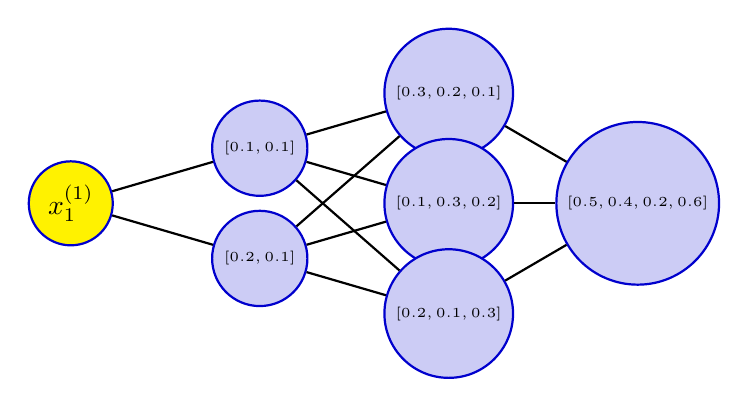
\begin{tikzpicture}[x=2.4cm,y=1.4cm]
  \readlist\Nnod{1, 2, 3, 1} % number of nodes per layer
  
  % Define weights for each layer
  % Layer 1 (input): no weights needed
  \readlist\Wone{{0.1, 0.1}, {0.2, 0.1}, {0.15, 0.2}} % weights for layer 2
  \readlist\Wtwo{{0.3, 0.2, 0.1}, {0.1, 0.3, 0.2}, {0.2, 0.1, 0.3}} % weights for layer 3
  \readlist\Wthree{{0.5, 0.4, 0.2, 0.6}} % weights for output layer

  % \Nnodlen = length of \Nnod (i.e. total number of layers)
  % \Nnod[1] = element (number of nodes) at index 1
  
  \foreachitem \N \in \Nnod{ % loop over layers
    % \N     = current element in this iteration (i.e. number of nodes for this layer)
    % \Ncnt  = index of current layer in this iteration
    \foreach \i [evaluate={\x=\Ncnt; \y=\N/2-\i+0.5; \prev=int(\Ncnt-1);}] in {1,...,\N}{ % loop over nodes
      \ifnum\Ncnt=1 % first layer (input layer)
        \node[mynode, fill=yellow] (N\Ncnt-\i) at (\x,\y) {$x_1^{(1)}$};
      \else\ifnum\Ncnt=2 % hidden layer (second layer)
        \node[mynode] (N\Ncnt-\i) at (\x,\y) {\tiny $[\Wone[\i]]$};
      \else\ifnum\Ncnt=3 % third layer
        \node[mynode] (N\Ncnt-\i) at (\x,\y) {\tiny $[\Wtwo[\i]]$};
      \else % output layer
        \node[mynode] (N\Ncnt-\i) at (\x,\y) {\tiny $[\Wthree[\i]]$};
      \fi\fi\fi
      
      \ifnum\Ncnt>1 % connect to previous layer
        \foreach \j in {1,...,\Nnod[\prev]}{ % loop over nodes in previous layer
          \draw[thick] (N\prev-\j) -- (N\Ncnt-\i); % connect arrows directly
        }
      \fi % else: nothing to connect first layer
    }
  }
\end{tikzpicture}

\end{center}
Each neuron is a denoted by circle consisting of affine part (Linear Model) and activation function.

\begin{enumerate}
\item Single feature, the first layer contains two neurons, one hidden layer with three neurons, and one  output.
\item Consider classification problem either 0 or 1.
\item Superscript $(1)$ means first training sample, subscript $1$ feature index. 
\item Intermediate nodes $\wbf = [w_0, w_1, \ldots]$.
\end{enumerate}

\end{frame}

\begin{frame}{Forward Propagation}
Consider the first training sample $x_1^{(1)} = 2.0$. True label as $1$. Also consider Sigmoid as the activation function, i.e. $\sigma(z) = \frac{1}{1+e^{-z}}$.

Layer 1: 
\begin{enumerate}

\item Neuron 1: $z_1^{[1]} = 0.1 + 0.1\times2.0 = 0.3$. $a_1^{[1]} =  \frac{1}{1+e^{-0.3}}  = 0.5744$.

\item Neuron 2: $z_2^{[1]} = 0.2 + 0.1\times2.0 = 0.4$. $a_2^{[1]} =  \frac{1}{1+e^{-0.4}}  = 0.5987$.

\end{enumerate} 

Here, in an essence, the first layer expands one feature to two features, and basically each neurons will learn something different from the training data.
\end{frame}


\begin{frame}{Forward Propagation}

Layer 2:

\begin{enumerate}
\item Neuron 1: $z_1^{[2]} = 0.3 + 0.2 \times 0.5744 + 0.1 \times 0.5987 =  0.4748$. $a_1^{[2]} = \sigma(0.4748) = 0.6165$.

\item Neuron 2: $z_2^{[2]} = 0.1 + 0.3 \times 0.5744 + 0.2 \times 0.5987 = 0.3921$. $a_2^{[2]} = \sigma( 0.3921) = 0.5968$.

\item Neuron 3: $z_3^{[2]} = 0.2 + 0.1 \times 0.5744 + 0.3 \times 0.5987 =  0.4371$. $a_3^{[2]} = \sigma( 0.4371) = 0.6076$.
\end{enumerate}

\end{frame}

\begin{frame}{Forward Propagation}

Layer 3 (Output):

\begin{enumerate}
\item Output Neuron: $z_1^{[3]} = 0.5 + 0.4 \times 0.6165 + 0.2 \times 0.5968 + 0.6 \times 0.6075 = 1.2305$.
\item $a_1^{[3]} = \sigma(1.2305) =  0.7739$.
\end{enumerate}

The final output $\hat{y} =  0.7739$.
\end{frame}


\begin{frame}{Cross-Entropy Loss Calculation}
Given the true label $y = 1$ and predicted output $\hat{y} = 0.7739$:

\begin{align*}
\text{Cross-Entropy Loss} &= -[y \log(\hat{y}) + (1-y) \log(1-\hat{y})] \\
&= -[1 \cdot \log(0.7739) + 0 \cdot \log(1-0.7739)] \\
&= -\log(0.7739) \\
&= -(-0.2563) \\
&= 0.2563
\end{align*}

Where $\log$ denotes natural logarithm, and $\log(0.7740) \approx -0.2563$.

\vspace{0.5cm}

\begin{itemize}
\item The loss quantifies how well the network's prediction matches the true label.
\item Lower loss indicates better prediction (perfect prediction would give loss = 0).
\item For binary classification with sigmoid activation, cross-entropy loss is commonly used.
\end{itemize}
\end{frame}


\begin{frame}{Cross-Entropy Loss and Its Derivative}
For binary classification with true label $y \in \{0,1\}$ and predicted probability $\hat{y} \in (0,1)$, the cross-entropy loss is:

\begin{align*}
L(y, \hat{y}) &= -[y \log(\hat{y}) + (1-y) \log(1-\hat{y})]
\end{align*}

\textbf{Its derivative:}
\begin{align*}
\frac{\partial L}{\partial \hat{y}} &= \frac{\partial}{\partial \hat{y}}[-y \log(\hat{y}) - (1-y)\log(1-\hat{y})] \\
&= -y \cdot \frac{1}{\hat{y}} \cdot 1 - (1-y) \cdot \frac{1}{1-\hat{y}} \cdot (-1) \\
&= -\frac{y}{\hat{y}} + \frac{1-y}{1-\hat{y}}
\end{align*}

\footnotesize

\begin{itemize}
\item When $y=1$: $\frac{\partial L}{\partial \hat{y}} = -\frac{1}{\hat{y}} + 0 = -\frac{1}{\hat{y}}$
\item When $y=0$: $\frac{\partial L}{\partial \hat{y}} = 0 + \frac{1}{1-\hat{y}} = \frac{1}{1-\hat{y}}$
\item The gradient encourages $\hat{y}$ to move toward $y$ (negative gradient pushes $\hat{y}$ up when $y=1$)
\end{itemize}
\end{frame}

\begin{frame}{Sigmoid Activation Function and Its Derivative}
The sigmoid function and its derivative have a nice property:

\begin{align*}
\sigma(z) &= \frac{1}{1 + e^{-z}} = \hat{y} \\
\frac{d\sigma}{dz} &= \sigma(z)[1 - \sigma(z)] = \hat{y}(1-\hat{y})
\end{align*}

\tiny

\textbf{Derivation:}
\begin{align*}
\frac{d\sigma}{dz} &= \frac{d}{dz}\left(1 + e^{-z}\right)^{-1} \\
&= -(1 + e^{-z})^{-2} \cdot (-e^{-z}) \\
&= \frac{e^{-z}}{(1 + e^{-z})^2} \\
&= \frac{1}{1 + e^{-z}} \cdot \frac{e^{-z}}{1 + e^{-z}} \\
&= \sigma(z) \cdot \left(1 - \frac{1}{1 + e^{-z}}\right) \\
&= \sigma(z)[1 - \sigma(z)]
\end{align*}

 The derivative is expressed in terms of the function value itself . No need to recompute $e^{-z}$.
\end{frame}

\begin{frame}{Chain Rule in Backpropagation}
Backpropagation uses the chain rule from calculus:

If $L = f(g(h(x)))$, then:
\begin{align*}
\frac{\partial L}{\partial x} &= \frac{\partial L}{\partial f} \cdot \frac{\partial f}{\partial g} \cdot \frac{\partial g}{\partial h} \cdot \frac{\partial h}{\partial x}
\end{align*}

\tiny 

\textbf{In Neural Networks:}
\begin{align*}
L &\leftarrow \text{Loss function} \\
\hat{y} &\leftarrow \sigma(z^{[\ell]}) \quad \text{(output activation)}, \ell \text{~denotes layer index} \\
z^{[\ell]} &\leftarrow w^{[\ell]}a^{[\ell-1]} + w_0^{[\ell]} \quad \text{(linear combination)} \\
a^{[\ell-1]} &\leftarrow \sigma(z^{[\ell-1]}) \quad \text{(previous layer activation)}
\end{align*}


\textbf{Gradient flow:}
\begin{align*}
\frac{\partial L}{\partial w^{[\ell]}} &= \frac{\partial L}{\partial \hat{y}} \cdot \frac{\partial \hat{y}}{\partial z^{[\ell]}} \cdot \frac{\partial z^{[\ell]}}{\partial w^{[\ell]}} \\
&= \left(-\frac{y}{\hat{y}} + \frac{1-y}{1-\hat{y}}\right) \cdot \hat{y}(1-\hat{y}) \cdot a^{[\ell-1]}
\end{align*}

\textbf{Note:} $\hat{y}(1-\hat{y})$ cancels when $\hat{y}$ is not 0 or 1, simplifying computation!
\end{frame}

\begin{frame}{These Derivatives Are Well-Behaved}

\footnotesize

\textbf{1. Numerical Stability:}
\begin{itemize}
\item Cross-entropy with sigmoid avoids extreme gradients
\item For $\hat{y} \approx 0$ or $\hat{y} \approx 1$: $\hat{y}(1-\hat{y}) \approx 0$
\item This prevents huge weight updates when confident but wrong
\end{itemize}

\textbf{2. Gradient Behavior:}
\begin{align*}
\frac{\partial L}{\partial z^{[\ell]}} &= \hat{y} - y \quad \text{(after simplification!)}
\end{align*}

\textbf{Derivation:}
\begin{align*}
\frac{\partial L}{\partial z^{[\ell]}} &= \left(-\frac{y}{\hat{y}} + \frac{1-y}{1-\hat{y}}\right) \cdot \hat{y}(1-\hat{y}) \\
&= -y(1-\hat{y}) + (1-y)\hat{y} = -y + y\hat{y} + \hat{y} - y\hat{y} = \hat{y} - y
\end{align*}

\textbf{Beautiful Result:} The gradient is simply the prediction error!
\begin{itemize}
\item When $\hat{y} > y$: Positive gradient decreases weights
\item When $\hat{y} < y$: Negative gradient increases weights
\item Intuitive and numerically stable
\end{itemize}
\end{frame}


\begin{frame}{Backpropagation: Gradient Calculation}
We'll compute gradients using chain rule. Recall: $\hat{y} = 0.7740$, $y = 1$.

\vspace{0.3cm}

\textbf{Step 1: Output Layer Gradient}
\begin{align*}
\frac{\partial L}{\partial \hat{y}} &= -\frac{y}{\hat{y}} + \frac{1-y}{1-\hat{y}} = -\frac{1}{0.7740} + 0 = -1.2921 \\
\frac{\partial \hat{y}}{\partial z^{[3]}} &= \hat{y}(1-\hat{y}) = 0.7739 \times  0.2261 =  0.1750
  \\
\frac{\partial L}{\partial z^{[3]}} &= \frac{\partial L}{\partial \hat{y}} \cdot \frac{\partial \hat{y}}{\partial z^{[3]}} = -1.2922 \times  0.1750 = -0.2261
\end{align*}

\end{frame}


\begin{frame}{Backpropagation: Gradient Calculation}

\textbf{Step 2: Layer 3 Weight Gradients}
\begin{align*}
\frac{\partial z^{[3]}}{\partial w_0^{[3]}} &= 1, \quad
\frac{\partial L}{\partial w_0^{[3]}} = -0.2261 \times 1 = -0.2261 \\
\frac{\partial z^{[3]}}{\partial w_1^{[3]}} &= a_1^{[2]} = 0.6165, \quad
\frac{\partial L}{\partial w_1^{[3]}} = -0.2261 \times 0.6165 = -0.1394 \\
\frac{\partial z^{[3]}}{\partial w_2^{[3]}} &= a_2^{[2]} = 0.5968, \quad
\frac{\partial L}{\partial w_2^{[3]}} = -0.2261 \times 0.5968 = -0.1349 \\
\frac{\partial z^{[3]}}{\partial w_3^{[3]}} &= a_3^{[2]} = 0.6075, \quad
\frac{\partial L}{\partial w_3^{[3]}} = -0.2261 \times 0.6075 = -0.1374
\end{align*}
\end{frame}

\begin{frame}{Backpropagation: Layer 2 Gradients}
\textbf{Step 3: Backpropagate to Layer 2}
\begin{align*}
\frac{\partial L}{\partial a_1^{[2]}} &= \frac{\partial L}{\partial z^{[3]}} \cdot \frac{\partial z^{[3]}}{\partial a_1^{[2]}} = -0.2261 \times 0.4 = -0.0904 \\
\frac{\partial L}{\partial a_2^{[2]}} &= -0.2261 \times 0.2 = -0.0452 \\
\frac{\partial L}{\partial a_3^{[2]}} &= -0.2261 \times 0.6 = -0.1357
\end{align*}

\end{frame}


\begin{frame}{Backpropagation: Gradient Calculation}

\small

\textbf{Step 4: Layer 2 Neuron Gradients}
For each neuron $i$ in layer 2: $\frac{\partial a_i^{[2]}}{\partial z_i^{[2]}} = a_i^{[2]}(1-a_i^{[2]})$
\begin{align*}
\frac{\partial L}{\partial z_1^{[2]}} &= \frac{\partial L}{\partial a_1^{[2]}} \cdot a_1^{[2]}(1-a_1^{[2]}) = -0.0904 \times (0.6165 \times 0.3835) = -0.0904 \times 0.2364 = -0.0214 \\
\frac{\partial L}{\partial z_2^{[2]}} &= -0.0452 \times (0.5968 \times 0.4032) = -0.0452 \times 0.2406 = -0.0109 \\
\frac{\partial L}{\partial z_3^{[2]}} &= -0.1356 \times (0.6075 \times 0.3925) = -0.1356 \times 0.2384 = -0.0323
\end{align*}
\end{frame}

\begin{frame}{Backpropagation: Layer 2 Weight Gradients}

\footnotesize

\textbf{Step 5: Layer 2 Weight Gradients}
For neuron 1 in layer 2:
\begin{align*}
\frac{\partial L}{\partial w_{01}^{[2]}} &= \frac{\partial L}{\partial z_1^{[2]}} \times 1 = -0.0214 \\
\frac{\partial L}{\partial w_{11}^{[2]}} &= \frac{\partial L}{\partial z_1^{[2]}} \times a_1^{[1]} = -0.0214 \times 0.5744 = -0.0123 \\
\frac{\partial L}{\partial w_{21}^{[2]}} &= \frac{\partial L}{\partial z_1^{[2]}} \times a_2^{[1]} = -0.0214 \times 0.5987 = -0.0128
\end{align*}

For neuron 2 in layer 2:
\begin{align*}
\frac{\partial L}{\partial w_{02}^{[2]}} &= -0.0109, \quad
\frac{\partial L}{\partial w_{12}^{[2]}} = -0.0109 \times 0.5744 = -0.0063, \quad
\frac{\partial L}{\partial w_{22}^{[2]}} = -0.0109 \times 0.5987 = -0.0065
\end{align*}

For neuron 3 in layer 2:
\begin{align*}
\frac{\partial L}{\partial w_{03}^{[2]}} &= -0.0323, \quad
\frac{\partial L}{\partial w_{13}^{[2]}} = -0.0323 \times 0.5744 = -0.0186, \quad
\frac{\partial L}{\partial w_{23}^{[2]}} = -0.0323 \times 0.5987 = -0.0194
\end{align*}
\end{frame}

\begin{frame}{Backpropagation: Layer 1 Gradients}

\footnotesize

\textbf{Step 6: Backpropagate to Layer 1}
\begin{align*}
\frac{\partial L}{\partial a_1^{[1]}} &= \sum_{j=1}^3 \frac{\partial L}{\partial z_j^{[2]}} \cdot w_{1j}^{[2]} \\
&= (-0.0214 \times 0.2) + (-0.0109 \times 0.3) + (-0.0323 \times 0.1) \\
&= -0.00428 - 0.00327 - 0.00323 = -0.01078 \\
\frac{\partial L}{\partial a_2^{[1]}} &= (-0.0214 \times 0.1) + (-0.0109 \times 0.2) + (-0.0323 \times 0.3) \\
&= -0.00214 - 0.00218 - 0.00969 = -0.01401
\end{align*}

\textbf{Step 7: Layer 1 Neuron Gradients}
\begin{align*}
\frac{\partial L}{\partial z_1^{[1]}} &= \frac{\partial L}{\partial a_1^{[1]}} \cdot a_1^{[1]}(1-a_1^{[1]}) = -0.01078 \times (0.5744 \times 0.4256) = -0.01078 \times 0.2445 = -0.00264 \\
\frac{\partial L}{\partial z_2^{[1]}} &= -0.01401 \times (0.5987 \times 0.4013) = -0.01401 \times 0.2403 = -0.00337
\end{align*}
\end{frame}

\begin{frame}{Backpropagation: Layer 1 Weight Gradients}

\footnotesize

\textbf{Step 8: Layer 1 Weight Gradients}
For neuron 1 in layer 1 (input $x_1^{(1)} = 2.0$):
\begin{align*}
\frac{\partial L}{\partial w_{01}^{[1]}} &= \frac{\partial L}{\partial z_1^{[1]}} \times 1 = -0.00264 \\
\frac{\partial L}{\partial w_{11}^{[1]}} &= \frac{\partial L}{\partial z_1^{[1]}} \times x_1^{(1)} = -0.00264 \times 2.0 = -0.00528
\end{align*}

For neuron 2 in layer 1:
\begin{align*}
\frac{\partial L}{\partial w_{02}^{[1]}} &= \frac{\partial L}{\partial z_2^{[1]}} \times 1 = -0.00337 \\
\frac{\partial L}{\partial w_{12}^{[1]}} &= \frac{\partial L}{\partial z_2^{[1]}} \times x_1^{(1)} = -0.00337 \times 2.0 = -0.00674
\end{align*}

\vspace{0.3cm}

\textbf{We've computed all gradients needed for weight updates using gradient descent}:
$$\mathbf{w} \leftarrow \mathbf{w} - \eta \frac{\partial L}{\partial \mathbf{w}}$$
where $\eta$ is the learning rate.
\end{frame}

\begin{frame}{Weight Updates with Gradient Descent}

\footnotesize

Using gradient descent with learning rate $\eta = 0.1$ :

$$\mathbf{w}_{\text{new}} = \mathbf{w}_{\text{old}} - \eta \cdot \frac{\partial L}{\partial \mathbf{w}}$$

\textbf{Output Layer Updates:}
\begin{align*}
{w_0}^{[3]}_{\text{new}} &= 0.5 - 0.1 \times (-0.2261) = 0.5 + 0.0226 = 0.5226 \\
{w_1}^{[3]}_{\text{new}} &= 0.4 - 0.1 \times (-0.1393) = 0.4 + 0.01393 = 0.4139 \\
{w_2}^{[3]}_{\text{new}} &= 0.2 - 0.1 \times (-0.1349) = 0.2 + 0.01349 = 0.2135 \\
{w_3}^{[3]}_{\text{new}} &= 0.6 - 0.1 \times (-0.1373) = 0.6 + 0.01373 = 0.6137
\end{align*}
\end{frame}

\begin{frame}{Layer 2 Weight Updates}

\footnotesize


\textbf{Neuron 1 in Layer 2:}
\begin{align*}
w_{01}^{[2]_{\text{new}}} &= 0.3 - 0.1 \times (-0.0214) = 0.3 + 0.00214 = 0.3021 \\
w_{11}^{[2]_{\text{new}}} &= 0.2 - 0.1 \times (-0.0123) = 0.2 + 0.00123 = 0.2012 \\
w_{21}^{[2]_{\text{new}}} &= 0.1 - 0.1 \times (-0.0128) = 0.1 + 0.00128 = 0.1013
\end{align*}

\textbf{Neuron 2 in Layer 2:}
\begin{align*}
w_{02}^{[2]_{\text{new}}} &= 0.1 - 0.1 \times (-0.0109) = 0.1 + 0.00109 = 0.1011 \\
w_{12}^{[2]_{\text{new}}} &= 0.3 - 0.1 \times (-0.0063) = 0.3 + 0.00063 = 0.3006 \\
w_{22}^{[2]_{\text{new}}} &= 0.2 - 0.1 \times (-0.0065) = 0.2 + 0.00065 = 0.2007
\end{align*}

\textbf{Neuron 3 in Layer 2:}
\begin{align*}
w_{03}^{[2]_{\text{new}}} &= 0.2 - 0.1 \times (-0.0323) = 0.2 + 0.00323 = 0.2032 \\
w_{13}^{[2]_{\text{new}}} &= 0.1 - 0.1 \times (-0.0186) = 0.1 + 0.00186 = 0.1019 \\
w_{23}^{[2]_{\text{new}}} &= 0.3 - 0.1 \times (-0.0193) = 0.3 + 0.00193 = 0.3019
\end{align*}
\end{frame}

\begin{frame}{Layer 1 Weight Updates}

\footnotesize


\textbf{Neuron 1 in Layer 1:}
\begin{align*}
w_{01}^{[1]_{\text{new}}} &= 0.1 - 0.1 \times (-0.00264) = 0.1 + 0.000264 = 0.1003 \\
w_{11}^{[1]_{\text{new}}} &= 0.1 - 0.1 \times (-0.00528) = 0.1 + 0.000528 = 0.1005
\end{align*}

\textbf{Neuron 2 in Layer 1:}
\begin{align*}
w_{02}^{[1]_{\text{new}}} &= 0.2 - 0.1 \times (-0.00337) = 0.2 + 0.000337 = 0.2003 \\
w_{12}^{[1]_{\text{new}}} &= 0.1 - 0.1 \times (-0.00674) = 0.1 + 0.000674 = 0.1007
\end{align*}

\vspace{0.5cm}

\begin{itemize}
\item All weights increased slightly because gradients were negative
\item Negative gradient means loss decreases as weight increases
\item Largest updates: Output layer weights (especially bias $w_0^{[3]}$)
\item Smallest updates: First layer weights (vanishing gradient effect)
\item After one training step: Loss should decrease on next forward pass
\end{itemize}
\end{frame}

\begin{frame}{Verification: Forward Pass with New Weights}

\footnotesize


Let's verify the network improves by doing one forward pass with updated weights:

\textbf{Layer 1 with new weights:}
\begin{align*}
z_1^{[1]} &= 0.1003 + 0.1005 \times 2.0 = 0.3013 \quad & a_1^{[1]} &= 0.5748 \\
z_2^{[1]} &= 0.2003 + 0.1007 \times 2.0 = 0.4017 \quad & a_2^{[1]} &= 0.5991
\end{align*}

\textbf{Layer 2 with new weights:}
\begin{align*}
z_1^{[2]} &= 0.3021 + 0.2012 \times 0.5748 + 0.1013 \times 0.5991 = 0.4785 \quad & a_1^{[2]} &= 0.6174 \\
z_2^{[2]} &= 0.1011 + 0.3006 \times 0.5748 + 0.2007 \times 0.5991 = 0.3941 \quad & a_2^{[2]} &= 0.5973 \\
z_3^{[2]} &= 0.2032 + 0.1019 \times 0.5748 + 0.3019 \times 0.5991 = 0.4427 \quad & a_3^{[2]} &= 0.6089
\end{align*}

\textbf{Output Layer with new weights:}
\begin{align*}
z_1^{[3]} &= 0.5226 + 0.4139 \times 0.6147 + 0.2135 \times 0.5973 + 0.6137 \times 0.6089 = 1.2794 \\
\hat{y}_{\text{new}} &= \sigma(1.2794) = 0.7823
\end{align*}
\end{frame}

\begin{frame}{Verification: New Loss Calculation}

\footnotesize


Original prediction: $\hat{y} = 0.7739$, New prediction: $\hat{y}_{\text{new}} = 0.7823$

\textbf{Original Loss:}
$$L = -\log(0.7739) = 0.2563$$

\textbf{New Loss:}
$$L_{\text{new}} = -\log(0.7823) = 0.2455$$

\vspace{0.5cm}

\textbf{Improvement:}
$$\Delta L = 0.2563 - 0.2455 = 0.0108 \quad \text{(4.23\% reduction)}$$

\vspace{0.5cm}

\textbf{Observations:}
\begin{itemize}
\item The network output increased from 0.7739 to 0.7823 (closer to target 1.0)
\item Loss decreased from 0.2563 to 0.2455
\item Gradient descent successfully reduced the loss
\item Multiple epochs (repetitions) would further optimize weights
\end{itemize}

\textbf{Learning Progress:} The network is learning to better predict the true label!
\end{frame}

\begin{frame}{Updated Network Visualization}
\begin{center}
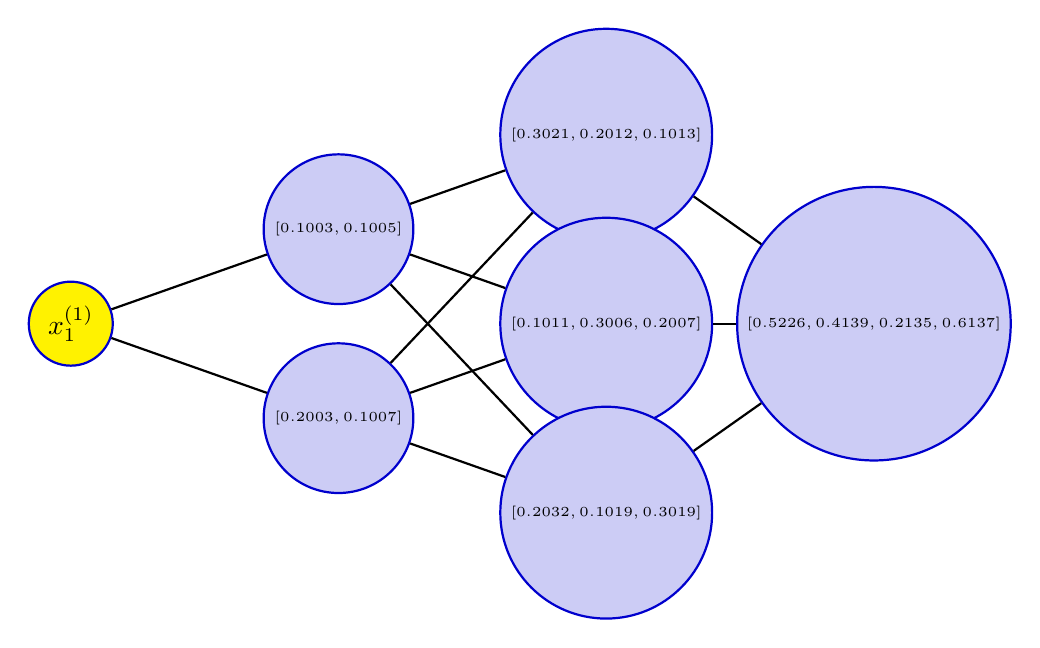
\begin{tikzpicture}[x=3.4cm,y=2.4cm]
  \readlist\Nnod{1, 2, 3, 1}
  
  % Updated weights after one gradient descent step
  \readlist\Wone{{0.1003, 0.1005}, {0.2003, 0.1007}} % Layer 1
  \readlist\Wtwo{{0.3021, 0.2012, 0.1013}, {0.1011, 0.3006, 0.2007}, {0.2032, 0.1019, 0.3019}} % Layer 2
  \readlist\Wthree{{0.5226, 0.4139, 0.2135, 0.6137}} % Output layer
  
  \foreachitem \N \in \Nnod{
    \foreach \i [evaluate={\x=\Ncnt; \y=\N/2-\i+0.5; \prev=int(\Ncnt-1);}] in {1,...,\N}{
      \ifnum\Ncnt=1
        \node[mynode, fill=yellow] (N\Ncnt-\i) at (\x,\y) {$x_1^{(1)}$};
      \else\ifnum\Ncnt=2
        \node[mynode] (N\Ncnt-\i) at (\x,\y) {\tiny $[\Wone[\i]]$};
      \else\ifnum\Ncnt=3
        \node[mynode] (N\Ncnt-\i) at (\x,\y) {\tiny $[\Wtwo[\i]]$};
      \else
        \node[mynode] (N\Ncnt-\i) at (\x,\y) {\tiny $[\Wthree[\i]]$};
      \fi\fi\fi
      
      \ifnum\Ncnt>1
        \foreach \j in {1,...,\Nnod[\prev]}{
          \draw[thick] (N\prev-\j) -- (N\Ncnt-\i);
        }
      \fi
    }
  }
\end{tikzpicture}
\end{center}

\end{frame}

\begin{frame}{At the end of first iteration:}

\begin{itemize}
\item All weights slightly increased (negative gradients)
\item Output layer bias $w_0^{[3]}$ increased most (0.5 → 0.5226)
\item First layer weights changed minimally (vanishing gradient)
\item Network now predicts 0.7862 (improved from 0.7740)
\end{itemize}

\textbf{Next Steps:} Repeat process for entire training dataset over many epochs!
\end{frame}



\section{A Brief Matrix Calculus}

\begin{frame}
    \sectionpage
\end{frame}


\begin{frame}{Derivatives in Neural Network Training}

\begin{enumerate}
\item Training means choose suitable $\wbf$ iteratively.
\item i.e. minimizing a loss function.
\end{enumerate}


Minimize loss $\to$ Gradient Descent $\to$ partial derivative wrt $\wbf$.

\vspace{10pt}

$\wbf$ is a vector.

For neuron, scalar version can work, for multiple neurons, and multiple inputs, it is cumbersome, we need a better frame work, aka Matrix!

\end{frame}


\begin{frame}{Gradient}

\begin{tblock}{Definition}
Vector of partial derivatives:

\begin{align*}
\nabla f (x, y) = \bigg[ \frac{\partial f(x,y)}{\partial x}, \frac{\partial f(x,y)}{\partial y} \bigg]
\end{align*}

This is about vector calculus, but in a Neural Network, we not only have one function of many variables but many functions of many variables, $\to$ Matrix calculus.

\end{tblock}

\end{frame}


\begin{frame}{Jacobian}

If we have two functions $f$ and $g$, 

then 

\begin{align*}
J = \begin{bmatrix}
\nabla f (x, y) \\ \nabla g (x, y) 
\end{bmatrix} = \begin{bmatrix}
\frac{\partial f(x,y)}{\partial x} & \frac{\partial f(x,y)}{\partial y}\\\frac{\partial g(x,y)}{\partial x} &\frac{\partial g(x,y)}{\partial y}
\end{bmatrix}
\end{align*}

\end{frame}

\begin{frame}{Generalization}

Assume $f(x, y, z) \Rightarrow  f(\xbf) $ Or in general, $\xbf = \begin{bmatrix}
x_1 \\ x_2 \\ x_3 \\ x_4  \\ \vdots
\end{bmatrix}
$

$\bullet$ Scalar-valued functions can be written as vectors $\ybf = \fbf(\xbf)$.

So,

\begin{align*}
\frac{\partial \mathbf{y}}{\partial \mathbf{x}} = 
\begin{bmatrix}
\nabla f_1(\mathbf{x}) \\ \nabla f_2(\mathbf{x}) \\ \dots \\ \nabla f_m(\mathbf{x})
\end{bmatrix} = 
\begin{bmatrix}
\frac{\partial}{\partial \mathbf{x}} f_1(\mathbf{x}) \\ \frac{\partial}{\partial \mathbf{x}} f_2(\mathbf{x}) \\ \dots \\ \frac{\partial}{\partial \mathbf{x}} f_m(\mathbf{x})
\end{bmatrix} = 
\begin{bmatrix}
\frac{\partial}{\partial x_1} f_1(\mathbf{x}) & \frac{\partial}{\partial x_2} f_1(\mathbf{x}) & \dots & \frac{\partial}{\partial x_n} f_1(\mathbf{x}) \\ 
\frac{\partial}{\partial x_1} f_2(\mathbf{x}) & \frac{\partial}{\partial x_2} f_2(\mathbf{x}) & \dots & \frac{\partial}{\partial x_n} f_2(\mathbf{x}) \\ 
\dots & \dots & \dots & \dots \\ 
\frac{\partial}{\partial x_1} f_m(\mathbf{x}) & \frac{\partial}{\partial x_2} f_m(\mathbf{x}) & \dots & \frac{\partial}{\partial x_n} f_m(\mathbf{x})
\end{bmatrix}
\end{align*}

\end{frame}

\begin{frame}{Some Notes on Generalization}

\begin{itemize}
\item $\frac{\partial}{\partial \mathbf{x}} f_i(\mathbf{x}) $ is a horizontal (row) $n$-vector.
\item Width of Jacobian is $n$ and have $m$ rows.
\end{itemize}

\end{frame}


\begin{frame}{Classwork}

Derive the Jacobian of identify function $\fbf(\xbf) = \xbf $, i.e. $f_i(\xbf) = x_i$ that has $n$ functions and each function has $n$ parameters held in a single vector $\xbf$.

\end{frame}


\begin{frame}{Element-wise Binary Operators}
\begin{facts}{}
By "element-wise binary operations" we mean applying
an operator to the first item of each vector to get the first item of the output, then to the second items of the inputs for the second item of the output, and so forth.
\end{facts}

Element-wise binary operation: $\ybf = \fbf(\wbf) \bigcirc \gbf(\xbf)$

Consider $m = n$ for this case.

Essentially, in scalar format:

\begin{align*}
\begin{bmatrix}
y_1 \\ y_2 \\ \vdots \\ y_n
\end{bmatrix} = 
\begin{bmatrix}
f_1(\mathbf{w}) \bigcirc g_1(\mathbf{x}) \\ 
f_2(\mathbf{w}) \bigcirc g_2(\mathbf{x}) \\ 
\vdots \\ 
f_n(\mathbf{w}) \bigcirc g_n(\mathbf{x})
\end{bmatrix}
\end{align*}

Elementwise implies that $f_i$ is purely a function of $w_i$ and $g_i$ is purely a function of $x_i$.
\end{frame}



\begin{frame}{General Case of Element-wise Binary Operators}

Jacobian with respect to $\wbf$ can be expanded as 

\begin{align*}
J_{\mathbf{w}} = \frac{\partial \mathbf{y}}{\partial \mathbf{w}} = 
\begin{bmatrix}
\frac{\partial}{\partial w_1} (f_1(\mathbf{w}) \bigcirc g_1(\mathbf{x})) & \frac{\partial}{\partial w_2} (f_1(\mathbf{w}) \bigcirc g_1(\mathbf{x})) & \dots & \frac{\partial}{\partial w_n} (f_1(\mathbf{w}) \bigcirc g_1(\mathbf{x})) \\ 
\frac{\partial}{\partial w_1} (f_2(\mathbf{w}) \bigcirc g_2(\mathbf{x})) & \frac{\partial}{\partial w_2} (f_2(\mathbf{w}) \bigcirc g_2(\mathbf{x})) & \dots & \frac{\partial}{\partial w_n} (f_2(\mathbf{w}) \bigcirc g_2(\mathbf{x})) \\ 
\dots & \dots & \dots & \dots \\ 
\frac{\partial}{\partial w_1} (f_n(\mathbf{w}) \bigcirc g_n(\mathbf{x})) & \frac{\partial}{\partial w_2} (f_n(\mathbf{w}) \bigcirc g_n(\mathbf{x})) & \dots & \frac{\partial}{\partial w_n} (f_n(\mathbf{w}) \bigcirc g_n(\mathbf{x}))
\end{bmatrix}
\end{align*}

\end{frame}

\begin{frame}{General Case of Element-wise Binary Operators}

Jacobian with respect to $\xbf$ can be expanded as 

\begin{align*}
J_{\mathbf{x}} = \frac{\partial \mathbf{y}}{\partial \mathbf{x}} = 
\begin{bmatrix}
\frac{\partial}{\partial x_1} (f_1(\mathbf{w}) \bigcirc g_1(\mathbf{x})) & \frac{\partial}{\partial x_2} (f_1(\mathbf{w}) \bigcirc g_1(\mathbf{x})) & \dots & \frac{\partial}{\partial x_n} (f_1(\mathbf{w}) \bigcirc g_1(\mathbf{x})) \\ 
\frac{\partial}{\partial x_1} (f_2(\mathbf{w}) \bigcirc g_2(\mathbf{x})) & \frac{\partial}{\partial x_2} (f_2(\mathbf{w}) \bigcirc g_2(\mathbf{x})) & \dots & \frac{\partial}{\partial x_n} (f_2(\mathbf{w}) \bigcirc g_2(\mathbf{x})) \\ 
\dots & \dots & \dots & \dots \\ 
\frac{\partial}{\partial x_1} (f_n(\mathbf{w}) \bigcirc g_n(\mathbf{x})) & \frac{\partial}{\partial x_2} (f_n(\mathbf{w}) \bigcirc g_n(\mathbf{x})) & \dots & \frac{\partial}{\partial x_n} (f_n(\mathbf{w}) \bigcirc g_n(\mathbf{x}))
\end{bmatrix}
\end{align*}

The good news that most of the time, Jacobian will be a diagonal matrix that greatly simplifies the calculation!!



\end{frame}

\begin{frame}{Classwork}

\begin{redblock}{}
Under what conditions, are the off-diagonal elements of a Jacobian zero?
\end{redblock}

\end{frame}

\begin{frame}{Example}

Consider $\fbf(\wbf) = \wbf$ and $\gbf(\xbf) = \xbf$. $\fbf(\wbf) + \gbf(\xbf)$ has scalar equations $y_i = f_i(\wbf) + g_i(\xbf)$ which reduces to $y_i = f_i(w_i) + g_i(x_i) = w_i + x_i$. We can get partial derivatives as

\begin{align*}
\frac{\partial}{\partial w_i}(f_i(w_i) + g_i(x_i)) &= \frac{\partial}{\partial w_i}(w_i + x_i) = 1 + 0 = 1 \\
\frac{\partial}{\partial x_i}(f_i(w_i) + g_i(x_i)) &= \frac{\partial}{\partial x_i}(w_i + x_i) = 0 + 1 = 1
\end{align*}

This gives us $\frac{\partial (\wbf + \xbf)}{\partial \wbf} = \frac{\partial (\wbf + \xbf)}{\partial \xbf} = \Ibf$, the identity matrix.

\end{frame}

\begin{frame}{Results of Common Elementwise Binary Operations}
\begin{tabular}{|l|l|l|}
\hline
\textbf{Operation} & \textbf{Partial with respect to w} & \textbf{Result} \\ \hline
$+$ & $\frac{\partial(\mathbf{w}+\mathbf{x})}{\partial \mathbf{w}} = \text{diag}\left(\dots \frac{\partial(w_i+x_i)}{\partial w_i} \dots\right) = \text{diag}(\vec{1})$ & $I$ \\ \hline
$-$ & $\frac{\partial(\mathbf{w}-\mathbf{x})}{\partial \mathbf{w}} = \text{diag}\left(\dots \frac{\partial(w_i-x_i)}{\partial w_i} \dots\right) = \text{diag}(\vec{1})$ & $I$ \\ \hline
$\otimes$ & $\frac{\partial(\mathbf{w} \otimes \mathbf{x})}{\partial \mathbf{w}} = \text{diag}\left(\dots \frac{\partial(w_i \times x_i)}{\partial w_i} \dots\right)$ & $\text{diag}(\mathbf{x})$ \\ \hline
$\oslash$ & $\frac{\partial(\mathbf{w} \oslash \mathbf{x})}{\partial \mathbf{w}} = \text{diag}\left(\dots \frac{\partial(w_i / x_i)}{\partial w_i} \dots\right)$ & $\text{diag}\left(\dots \frac{1}{x_i} \dots\right)$ \\ \hline
\end{tabular}

\vspace{5pt}

$\otimes$ is also called the Hadamard product.
\end{frame}


\begin{frame}{Vector-Scalar Operation}

What about adding scalar $z$ to vector $\xbf$? 

\pause

\vspace{10pt}

$z$ gets expanded to vector with appropriate length to add to elements of $\xbf$.


\vspace{10pt}

In essence, 

\begin{align*}
z = \gbf(z) = \vec{1}z\\
\ybf  = \fbf(\xbf) + \gbf(z)
\end{align*}

\pause 

\vspace{10pt}

And then you can apply our previous discussion. $\vec{1}$ means a vertical vector (column vector of all 1s).


\vspace{10pt}

\textbf{Note:} Computing the partial derivative with respect to the scalar parameter however results in a vertical vector and not a diagonal matrix.




\end{frame}

\begin{frame}{Vector Sum Reduction and Calculus}

Consider
\begin{facts}{}
$y = \sum_{i=1}^n f_i(\xbf)$
\end{facts}
The sume is over the results of the function, and not the parameter itself. Then, 

\begin{align*}
\frac{\partial y}{\partial \mathbf{x}} &= \left[ \frac{\partial y}{\partial x_1}, \frac{\partial y}{\partial x_2}, \dots, \frac{\partial y}{\partial x_n} \right] \\
&= \left[ \frac{\partial}{\partial x_1} \sum_i f_i(\mathbf{x}), \frac{\partial}{\partial x_2} \sum_i f_i(\mathbf{x}), \dots, \frac{\partial}{\partial x_n} \sum_i f_i(\mathbf{x}) \right] \\
&= \left[ \sum_i \frac{\partial f_i(\mathbf{x})}{\partial x_1}, \sum_i \frac{\partial f_i(\mathbf{x})}{\partial x_2}, \dots, \sum_i \frac{\partial f_i(\mathbf{x})}{\partial x_n} \right] \quad \text{(move derivative inside } \Sigma)
\end{align*}

\end{frame}


\begin{frame}{Single Variable Chain Rule}

\begin{tcolorbox}
\begin{align*}
 y  & = f(g(x))\\
 y' &  = f'(g(x))g'(x)
\end{align*}
\end{tcolorbox}


We also rewrite by introducing an intermediate variable  $ u = g(x)$, so 

\begin{tcolorbox}[colframe=nuaalightblue, colback = red!10]
\begin{align*}
\frac{dy}{dx} = \frac{dy}{du} \frac{du}{dx}
\end{align*}
\end{tcolorbox}

Example: Use chain rule for $ \sin(x^2)$ to find its derivative wrt $x$.

\end{frame}


\begin{frame}{Law of Total Derivatives}

\begin{tcolorbox}[colback=nuaalightblue!10, colframe=red!30]
To compute $\frac{dy}{dx}$, we need to sum up all possible contributions from changes in $x$ to the change in $y$.
\end{tcolorbox}

Assume $ u_1 = g(x)$, and $ y = f(x) = u_2(x, u_1)$, then 


\begin{tcolorbox}[colframe=nuaalightblue, colback = red!10]
\begin{align*}
\frac{dy}{dx} = \frac{\partial f(x)}{\partial x} &= \frac{\partial u_2(x, u_1)}{\partial x} \\
&= \frac{\partial u_2}{\partial x} \frac{\partial x}{\partial x} + \frac{\partial u_2}{\partial u_1} \frac{\partial u_1}{\partial x} \\
&= \frac{\partial u_2}{\partial x} + \frac{\partial u_2}{\partial u_1} \frac{\partial u_1}{\partial x}
\end{align*}
\end{tcolorbox}


\end{frame}


\begin{frame}{Law of Total Derivatives}

In general

\begin{tcolorbox}[colframe=forestBlush, colback = red!10!yellow!10]

\begin{align*}
\frac{\partial f(x, u_1, \dots, u_n)}{\partial x} &= \frac{\partial f}{\partial x} + \frac{\partial f}{\partial u_1} \frac{\partial u_1}{\partial x} + \frac{\partial f}{\partial u_2} \frac{\partial u_2}{\partial x} + \dots + \frac{\partial f}{\partial u_n} \frac{\partial u_n}{\partial x} \\
&= \frac{\partial f}{\partial x} + \sum_{i=1}^n \frac{\partial f}{\partial u_i} \frac{\partial u_i}{\partial x}
\end{align*}
\end{tcolorbox}

This is called \textbf{\color{DarkGreen}Single-variable Total-derivative Chain Rule}.

\vspace{10pt}

The total derivative assumes all variables are potentially codependent whereas the partial derivative
assumes all variables but x are constants.

\vspace{5pt}

\textit{\color{crimson}Could we simplify the above expression further?}

\end{frame}

\begin{frame}{Vector Chain Rule}

\begin{align*}
\begin{bmatrix}
y_1(x) \\ 
y_2(x)
\end{bmatrix} = \begin{bmatrix}
f_1(x) \\ 
f_2(x)
\end{bmatrix} = \begin{bmatrix}
ln(x^2) \\ 
sin(3x)
\end{bmatrix}
\end{align*}


Consider $\ybf = \fbf(\gbf(x))$ with $g_1$ and $g_2$ as two intermediate variables: 

\begin{align*}
\begin{bmatrix}
g_1(x) \\ 
g_2(x)
\end{bmatrix} &= \begin{bmatrix}
x^2 \\ 
3x
\end{bmatrix} \\
\begin{bmatrix}
f_1(\mathbf{g}) \\ 
f_2(\mathbf{g})
\end{bmatrix} &= \begin{bmatrix}
ln(g_1) \\ 
sin(g_2)
\end{bmatrix}
\end{align*}

\begin{align*}
\frac{\partial \mathbf{y}}{\partial x} = \begin{bmatrix}
\frac{\partial f_1(\mathbf{g})}{\partial x} \\ 
\frac{\partial f_2(\mathbf{g})}{\partial x}
\end{bmatrix} &= \begin{bmatrix}
\frac{\partial f_1}{\partial g_1} \frac{\partial g_1}{\partial x} + \frac{\partial f_1}{\partial g_2} \frac{\partial g_2}{\partial x} \\ 
\frac{\partial f_2}{\partial g_1} \frac{\partial g_1}{\partial x} + \frac{\partial f_2}{\partial g_2} \frac{\partial g_2}{\partial x}
\end{bmatrix} = \begin{bmatrix}
\frac{1}{g_1} 2x + 0 \\ 
0 + \cos(g_2)3
\end{bmatrix} = \begin{bmatrix}
\frac{2x}{x^2} \\ 
3\cos(3x)
\end{bmatrix} = \begin{bmatrix}
\frac{2}{x} \\ 
3\cos(3x)
\end{bmatrix}
\end{align*}

\end{frame}


\begin{frame}{Vector Chain Rule}

Still, the goal is convert group of scalar operations into a vector operations.

\begin{align*}
\begin{bmatrix}
\frac{\partial f_1}{\partial g_1} \frac{\partial g_1}{\partial x} + \frac{\partial f_1}{\partial g_2} \frac{\partial g_2}{\partial x} \\ 
\frac{\partial f_2}{\partial g_1} \frac{\partial g_1}{\partial x} + \frac{\partial f_2}{\partial g_2} \frac{\partial g_2}{\partial x}
\end{bmatrix}
\end{align*}

could be written as 

\begin{align*}
\begin{bmatrix}
\frac{\partial f_1}{\partial g_1} & \frac{\partial f_1}{\partial g_2} \\ 
\frac{\partial f_2}{\partial g_1} & \frac{\partial f_2}{\partial g_2}
\end{bmatrix} \begin{bmatrix}
\frac{\partial g_1}{\partial x} \\ 
\frac{\partial g_2}{\partial x}
\end{bmatrix} \stackrel{\text{set}}{=} \frac{\partial \mathbf{f}}{\partial \mathbf{g}} \frac{\partial \mathbf{g}}{\partial x}
\end{align*}

by matrix multiplication. So the Jacobian is the multiplication of two other Jacobians.

\end{frame}

\begin{frame}{Vector Chain Rule}

Instead of a scalar $x$, if we consider $\mathbf{x}$, 

\begin{tcolorbox}{colback=powderGreen, colframe=cpelime}
\begin{align*}
\frac{\partial}{\partial \mathbf{x}} \mathbf{f}(\mathbf{g}(\mathbf{x})) = \frac{\partial \mathbf{f}}{\partial \mathbf{g}} \frac{\partial \mathbf{g}}{\partial \mathbf{x}} 
\end{align*}
\textbf{Note:} matrix multiply doesn't commute; order of  $\frac{\partial \mathbf{f}}{\partial \mathbf{g}} \frac{\partial \mathbf{g}}{\partial \mathbf{x}}$ matters.
\end{tcolorbox}

\end{frame}

\begin{frame}{Vector Chain Rule}

Expanding $\frac{\partial}{\partial \mathbf{x}} \mathbf{f}(\mathbf{g}(\mathbf{x})) $, 

\begin{align*}
\frac{\partial}{\partial \mathbf{x}}\mathbf{f}(\mathbf{g}(\mathbf{x})) = \begin{bmatrix}
\frac{\partial f_1}{\partial g_1} & \frac{\partial f_1}{\partial g_2} & \dots & \frac{\partial f_1}{\partial g_k} \\ 
\frac{\partial f_2}{\partial g_1} & \frac{\partial f_2}{\partial g_2} & \dots & \frac{\partial f_2}{\partial g_k} \\ 
\vdots & \vdots & \ddots & \vdots \\ 
\frac{\partial f_m}{\partial g_1} & \frac{\partial f_m}{\partial g_2} & \dots & \frac{\partial f_m}{\partial g_k}
\end{bmatrix} \begin{bmatrix}
\frac{\partial g_1}{\partial x_1} & \frac{\partial g_1}{\partial x_2} & \dots & \frac{\partial g_1}{\partial x_n} \\ 
\frac{\partial g_2}{\partial x_1} & \frac{\partial g_2}{\partial x_2} & \dots & \frac{\partial g_2}{\partial x_n} \\ 
\vdots & \vdots & \ddots & \vdots \\ 
\frac{\partial g_k}{\partial x_1} & \frac{\partial g_k}{\partial x_2} & \dots & \frac{\partial g_k}{\partial x_n}
\end{bmatrix}
\end{align*}

where $m = |f|$, $n = |x|$, and $k = |g|$, the resulting Jacobian matrix has dimensions $m \times n$ (derived from the multiplication of an $m \times k$ matrix by a $k \times n$ matrix). $|\cdot |$ denotes cardinality.


\vspace{15pt}

\textit{\color{red!80}When will the off-diagonal entries be zero for both matrices? How does that simplify our calculations?}

\end{frame}


\section{Matrix Calculus in Action}

\begin{frame}
    \sectionpage
\end{frame}

\begin{frame}{Gradient of Neuron Activation}


 We consider ReLU activation for simplicity.
 
 \begin{align*}
 activation(x) = max(0, \wbf \cdot \xbf + b)
 \end{align*}
 
 Focusing on $\pdv{(\wbf \cdot \xbf + b)}{\wbf}$, the dot product $\wbf \cdot \xbf$ is elementwise multiplication that can be written as $sum (\wbf \otimes \xbf)$.
 
 \end{frame}
 
 \begin{frame}{Gradient of Neuron Activation}

 
 \begin{align*}
\bm{u} &= \bm{w} \otimes \bm{x} \\
y &= \text{sum}(\bm{u})
\end{align*}
 
 Once we've rephrased $y$, we recognize two subexpressions with known partial derivatives:

\begin{align*}
\frac{\partial \bm{u}}{\partial \bm{w}} &= \frac{\partial}{\partial \bm{w}} (\bm{w} \otimes \bm{x}) = \text{diag}(\bm{x}) \\
\frac{\partial y}{\partial \bm{u}} &= \frac{\partial}{\partial \bm{u}} \text{sum}(\bm{u}) = \bm{1}^T
\end{align*}


The vector chain rule says to multiply the partials:

$$\frac{\partial y}{\partial \bm{w}} = \frac{\partial y}{\partial \bm{u}} \frac{\partial \bm{u}}{\partial \bm{w}} = \bm{1}^T \text{diag}(\bm{x}) = \bm{x}^T$$


\end{frame}




\begin{frame}[fragile]
\frametitle{Verification via Scalar Expansion}

To check our results, we can grind the dot product down into a pure scalar function:

\begin{align*}
y &= \bm{w} \cdot \bm{x} = \sum_{i}^{n} (w_i x_i) \\
\frac{\partial y}{\partial w_j} &= \frac{\partial}{\partial w_j} \sum_i (w_i x_i) = \sum_i \frac{\partial}{\partial w_j} (w_i x_i) = \frac{\partial}{\partial w_j} (w_j x_j) = x_j
\end{align*}

\vspace{0.3cm}

Then:

$$\frac{\partial y}{\partial \bm{w}} = [x_1, \ldots, x_n] = \bm{x}^T$$

\vspace{0.5cm}

\textbf{Hooray!} Our scalar results match the vector chain rule results.

\end{frame}

\begin{frame}[fragile]
\frametitle{Full Linear Layer with Bias}

Now, let $y = \bm{w} \cdot \bm{x} + b$, the full expression within the $\max$ activation function call. We have two different partials to compute, but we don't need the chain rule:

\begin{align*}
\frac{\partial y}{\partial \bm{w}} &= \frac{\partial}{\partial \bm{w}} \bm{w} \cdot \bm{x} + \frac{\partial}{\partial \bm{w}} b = \bm{x}^T + \bm{0}^T = \bm{x}^T \\
\frac{\partial y}{\partial b} &= \frac{\partial}{\partial b} \bm{w} \cdot \bm{x} + \frac{\partial}{\partial b} b = 0 + 1 = 1
\end{align*}

\end{frame}

\begin{frame}{Including Nonlinearity of the Activation Function}
Let's tackle the partials of the neuron activation, $\max(0, \bm{w} \cdot \bm{x} + b)$. The use of the $\max(0, z)$ function call on scalar $z$ just says to treat all negative $z$ values as 0. 

\vspace{0.3cm}

The derivative of the max function is a piecewise function:
\begin{itemize}
\item When $z \leq 0$, the derivative is 0 because $z$ is a constant
\item When $z > 0$, the derivative of the max function is just the derivative of $z$, which is 1
\end{itemize}

\vspace{0.3cm}

\begin{align*}\frac{\partial}{\partial z} \max(0, z) = \begin{cases}
0 & z \leq 0 \\
\frac{dz}{dz} = 1 & z > 0
\end{cases}
\end{align*}

\end{frame}


\begin{frame}[fragile]
\frametitle{Broadcasting Functions Across Vectors}

An aside on broadcasting functions across scalars. When one or both of the $\max$ arguments are vectors, such as $\max(0, \bm{x})$, we broadcast the single-variable function $\max$ across the elements. This is an example of an element-wise unary operator. 

\vspace{0.3cm}



\begin{align*}
\max(0, \bm{x}) = \begin{bmatrix}
\max(0, x_1) \\
\max(0, x_2) \\
\vdots \\
\max(0, x_n)
\end{bmatrix}
\end{align*}

\end{frame}


\begin{frame}[fragile]
\frametitle{Derivative of Broadcast ReLU}

For the derivative of the broadcast version then, we get a vector of zeros and ones where:

\begin{align*}
\frac{\partial}{\partial x_i} \max(0, x_i) = \begin{cases}
0 & x_i \leq 0 \\
\frac{dx_i}{dx_i} = 1 & x_i > 0
\end{cases}
\end{align*}

\vspace{0.3cm}

\begin{align*}
\frac{\partial}{\partial \bm{x}} \max(0, \bm{x}) = \begin{bmatrix}
\frac{\partial}{\partial x_1} \max(0, x_1) \\
\frac{\partial}{\partial x_2} \max(0, x_2) \\
\vdots \\
\frac{\partial}{\partial x_n} \max(0, x_n)
\end{bmatrix}
\end{align*}

\end{frame}

\begin{frame}[fragile]
\frametitle{Applying the Chain Rule to Activation}

To get the derivative of the $\text{activation}(\bm{x})$ function, we need the chain rule because of the nested subexpression, $\bm{w} \cdot \bm{x} + b$. 

\vspace{0.3cm}

Following our process, let's introduce intermediate scalar variable $z$ to represent the affine function giving:

\begin{align*}
z(\bm{w}, b, \bm{x}) &= \bm{w} \cdot \bm{x} + b \\
\text{activation}(z) &= \max(0, z)
\end{align*}

\end{frame}


\begin{frame}[fragile]
\frametitle{Applying the Chain Rule to Activation}

\small


\begin{align*}
\frac{\partial \text{activation}}{\partial \bm{w}} = \frac{\partial \text{activation}}{\partial z} \frac{\partial z}{\partial \bm{w}}
\end{align*}

\vspace{0.3cm}

which we can rewrite as follows:

\begin{align*}
\frac{\partial \text{activation}}{\partial \bm{w}} = \begin{cases}
0 \cdot \frac{\partial z}{\partial \bm{w}} = \bm{0}^T & z \leq 0 \\
1 \cdot \frac{\partial z}{\partial \bm{w}} = \frac{\partial z}{\partial \bm{w}} = \bm{x}^T & z > 0 \quad \text{(we computed $\frac{\partial z}{\partial \bm{w}} = \bm{x}^T$ previously)}
\end{cases}
\end{align*}

\vspace{0.3cm}

and then substitute $z = \bm{w} \cdot \bm{x} + b$ back in:

\begin{align*}
\frac{\partial \text{activation}}{\partial \bm{w}} = \begin{cases}
\bm{0}^T & \bm{w} \cdot \bm{x} + b \leq 0 \\
\bm{x}^T & \bm{w} \cdot \bm{x} + b > 0
\end{cases}
\end{align*}


When the activation function clips affine function output $z$ to 0, the derivative is zero with respect to any weight $w_i$. When $z > 0$, it's as if the $\max$ function disappears and we get just the derivative of $z$ with respect to the weights.


\end{frame}

\begin{frame}[fragile]
\frametitle{Derivative with Respect to Bias}

Turning now to the derivative of the neuron activation with respect to $b$, we get:

\begin{align*}
\frac{\partial \text{activation}}{\partial b} = \begin{cases}
0 \cdot \frac{\partial z}{\partial b} = 0 & \bm{w} \cdot \bm{x} + b \leq 0 \\
1 \cdot \frac{\partial z}{\partial b} = 1 & \bm{w} \cdot \bm{x} + b > 0
\end{cases}
\end{align*}

\end{frame}


\begin{frame}{Gradient of Neural Network Loss}

Feature matrix: $X = [\xbf_1, \xbf_2, \xbf_3, \cdots, \xbf_N]^\top$


$\ybf = [y_1, y_2, \cdots, y_N]$.

where $y_i$ is a scalar.

\vspace{10pt}

Cost function:

\begin{align*}
C(\bm{w}, b, X, \bm{y}) = \frac{1}{N} \sum_{i=1}^{N} (y_i - \text{activation}(\bm{x}_i))^2 = \frac{1}{N} \sum_{i=1}^{N} (y_i - \max(0, \bm{w} \cdot \bm{x}_i + b))^2
\end{align*}



\end{frame}


\begin{frame}[fragile]{}

Following our chain rule process we introduce these intermediate variables:

\begin{align*}
u(\bm{w}, b, \bm{x}) &= \max(0, \bm{w} \cdot \bm{x} + b) \\
v(y, u) &= y - u \\
C(v) &= \frac{1}{N} \sum_{i=1}^{N} v^2
\end{align*}

\end{frame}

\begin{frame}{Gradient Computation}

Recall

\begin{align*}
\frac{\partial}{\partial \bm{w}} u(\bm{w}, b, \bm{x}) = \begin{cases}
\bm{0}^T & \bm{w} \cdot \bm{x} + b \leq 0 \\
\bm{x}^T & \bm{w} \cdot \bm{x} + b > 0
\end{cases}
\end{align*}

and

\begin{align*}
\frac{\partial v(y, u)}{\partial \bm{w}} = \frac{\partial}{\partial \bm{w}} (y - u) = \bm{0}^T \frac{\partial u}{\partial \bm{w}} = -\frac{\partial u}{\partial \bm{w}} = \begin{cases}
\bm{0}^T & \bm{w} \cdot \bm{x} + b \leq 0 \\
-\bm{x}^T & \bm{w} \cdot \bm{x} + b > 0
\end{cases}
\end{align*}

\end{frame}


\begin{frame}{Gradient Computation}

\begin{align*}
\frac{\partial C(v)}{\partial \bm{w}} = \frac{\partial}{\partial \bm{w}} \frac{1}{N} \sum_{i=1}^{N} v_i^2 = \frac{1}{N} \sum_{i=1}^{N} \frac{\partial}{\partial \bm{w}} v_i^2 = \frac{1}{N} \sum_{i=1}^{N} \frac{\partial v_i^2}{\partial v} \frac{\partial v}{\partial \bm{w}} = \frac{1}{N} \sum_{i=1}^{N} 2v_i \frac{\partial v}{\partial \bm{w}}
\end{align*}

\vspace{0.2cm}

\begin{align*}
= \frac{1}{N} \sum_{i=1}^{N} \begin{cases}
2v_i \bm{0}^T = \bm{0}^T & \bm{w} \cdot \bm{x}_i + b \leq 0 \\
-2v_i \bm{x}^T & \bm{w} \cdot \bm{x}_i + b > 0
\end{cases}
\end{align*}


\end{frame}



\begin{frame}{Gradient Computation}

\footnotesize

\begin{align*}
\frac{\partial C(v)}{\partial \bm{w}} = \frac{1}{N} \sum_{i=1}^{N} \begin{cases}
\bm{0}^T & \bm{w} \cdot \bm{x}_i + b \leq 0 \\
-2(y_i - u)\bm{x}_i^T & \bm{w} \cdot \bm{x}_i + b > 0
\end{cases} = \frac{1}{N} \sum_{i=1}^{N} \begin{cases}
\bm{0}^T & \bm{w} \cdot \bm{x}_i + b \leq 0 \\
-2(y_i - \max(0, \bm{w} \cdot \bm{x}_i + b))\bm{x}_i^T & \bm{w} \cdot \bm{x}_i + b > 0
\end{cases}
\end{align*}

\vspace{0.2cm}

\begin{align*}
= \frac{1}{N} \sum_{i=1}^{N} \begin{cases}
\bm{0}^T & \bm{w} \cdot \bm{x}_i + b \leq 0 \\
-2(y_i - (\bm{w} \cdot \bm{x}_i + b))\bm{x}_i^T & \bm{w} \cdot \bm{x}_i + b > 0
\end{cases} = \begin{cases}
\bm{0}^T & \bm{w} \cdot \bm{x}_i + b \leq 0 \\
-\frac{2}{N} \sum_{i=1}^{N} (y_i - (\bm{w} \cdot \bm{x}_i + b))\bm{x}_i^T & \bm{w} \cdot \bm{x}_i + b > 0
\end{cases}
\end{align*}

\vspace{0.2cm}

\begin{align*}
= \begin{cases}
\bm{0}^T & \bm{w} \cdot \bm{x}_i + b \leq 0 \\
\frac{2}{N} \sum_{i=1}^{N} (\bm{w} \cdot \bm{x}_i + b - y_i)\bm{x}_i^T & \bm{w} \cdot \bm{x}_i + b > 0
\end{cases}
\end{align*}


We can substitute an error term $e_i = \bm{w} \cdot \bm{x}_i + b - y_i$ yielding:

\begin{align*}
\frac{\partial C}{\partial \bm{w}} = \frac{2}{N} \sum_{i=1}^{N} e_i \bm{x}_i^T \quad \text{(for the nonzero activation case)}
\end{align*}

\end{frame}


\begin{frame}{Gradient Computation}



What about the bias?

Intermediate variables:

\begin{align*}
u(\bm{w}, b, \bm{x}) &= \max(0, \bm{w} \cdot \bm{x} + b) \\
v(y, u) &= y - u \\
C(v) &= \frac{1}{N} \sum_{i=1}^{N} v^2
\end{align*}


From previous result:


\begin{align*}
\frac{\partial u}{\partial b} = \begin{cases}
0 & \bm{w} \cdot \bm{x} + b \leq 0 \\
1 & \bm{w} \cdot \bm{x} + b > 0
\end{cases}
\end{align*}

\end{frame}


\begin{frame}{Gradient Computation for Bias}

For $v$, the partial is:

\begin{align*}
\frac{\partial v(y, u)}{\partial b} = \frac{\partial}{\partial b} (y - u) = 0 - \frac{\partial u}{\partial b} = -\frac{\partial u}{\partial b} = \begin{cases}
0 & \bm{w} \cdot \bm{x} + b \leq 0 \\
-1 & \bm{w} \cdot \bm{x} + b > 0
\end{cases}
\end{align*}

\end{frame}


\begin{frame}{Gradient Computation for Bias}

\footnotesize

\begin{align*}
\frac{\partial C(v)}{\partial b} = \frac{\partial}{\partial b} \frac{1}{N} \sum_{i=1}^{N} v_i^2 = \frac{1}{N} \sum_{i=1}^{N} \frac{\partial}{\partial b} v_i^2 = \frac{1}{N} \sum_{i=1}^{N} \frac{\partial v_i^2}{\partial v} \frac{\partial v}{\partial b}
\end{align*}

\vspace{0.2cm}

\begin{align*}
= \frac{1}{N} \sum_{i=1}^{N} 2v_i \frac{\partial v}{\partial b}
\end{align*}

\vspace{0.2cm}

\begin{align*}
= \frac{1}{N} \sum_{i=1}^{N} \begin{cases}
0 & \bm{w} \cdot \bm{x} + b \leq 0 \\
-2v_i & \bm{w} \cdot \bm{x} + b > 0
\end{cases}
\end{align*}

\end{frame}

\begin{frame}{Gradient Computation for Bias}


\begin{align*}
\frac{\partial C(v)}{\partial b} = \frac{1}{N} \sum_{i=1}^{N} \begin{cases}
0 & \bm{w} \cdot \bm{x} + b \leq 0 \\
-2(y_i - \max(0, \bm{w} \cdot \bm{x}_i + b)) & \bm{w} \cdot \bm{x} + b > 0
\end{cases}
\end{align*}

\vspace{0.2cm}

\begin{align*}
= \frac{1}{N} \sum_{i=1}^{N} \begin{cases}
0 & \bm{w} \cdot \bm{x} + b \leq 0 \\
2(\bm{w} \cdot \bm{x}_i + b - y_i) & \bm{w} \cdot \bm{x} + b > 0
\end{cases}
\end{align*}

\vspace{0.3cm}

\begin{align*}
= \begin{cases}
0 & \bm{w} \cdot \bm{x} + b \leq 0 \\
\frac{2}{N} \sum_{i=1}^{N} (\bm{w} \cdot \bm{x}_i + b - y_i) & \bm{w} \cdot \bm{x} + b > 0
\end{cases}
\end{align*}

\end{frame}


\begin{frame}[fragile]
\frametitle{Error Term Substitution for Bias Gradient}

As before, we can substitute an error term:

\begin{align*}
\frac{\partial C}{\partial b} = \frac{2}{N} \sum_{i=1}^{N} e_i \quad \text{(for the nonzero activation case)}
\end{align*}

where $e_i = \bm{w} \cdot \bm{x}_i + b - y_i$ is the prediction error.

\vspace{0.5cm}

\begin{alert}

The bias gradient is proportional to the mean prediction error across all samples when the neuron is active.


\end{alert}

\end{frame}

% ============================================================
\begin{frame}[fragile]
\frametitle{Scalar vs. Vectorized Operations}

\small

\begin{tabular}{l|l|l}
\textbf{Operation} & \textbf{Scalar (Loop)} & \textbf{Vectorized} \\
\hline
Affine transformation & $z_i = \bm{x}_i^T \bm{w} + b$ & $\bm{z} = X\bm{w} + b$ \\
& One sample at a time & All $n$ samples at once \\
\hline
Activation & $u_i = \max(0, z_i)$ & $\bm{u} = \max(0, \bm{z})$ \\
& Scalar function & Element-wise operation \\
\hline
Loss & $C = \frac{1}{N}\sum_i v_i^2$ & $C = \frac{1}{N}\|\bm{v}\|_2^2$ \\
& Accumulate in loop & Vectorized norm \\
\hline
Gradient $\bm{w}$ & $\frac{\partial C}{\partial w_j} = \frac{2}{N}\sum_i x_{ij} e_i$ & $\frac{\partial C}{\partial \bm{w}} = \frac{2}{N}X^T\bm{e}$ \\
& Nested loops & Single matrix product \\
\hline
Gradient $b$ & $\frac{\partial C}{\partial b} = \frac{2}{N}\sum_i e_i$ & $\frac{\partial C}{\partial b} = \frac{2}{N}\mathbf{1}^T\bm{e}$ \\
& Single loop & Dot product \\
\end{tabular}

$N$: Number of samples.

\end{frame}


\begin{frame}{References/Readings}

\footnotesize

\textbf{Mandatory Reading}

\begin{enumerate}
\item The Matrix Calculus You Need For Deep Learning \url{https://arxiv.org/pdf/1802.01528}
\end{enumerate}



\textbf{Recommended Reading}

\begin{enumerate}
\item \url{https://lrjconan.github.io/UBC-CPEN455-DL/assets/slides_2025/mlp.pdf}
\item \url{https://www.csie.ntu.edu.tw/~cjlin/papers/autodiff/autodiff.pdf}
\item \url{https://comp6248.ecs.soton.ac.uk/handouts/autograd-handouts.pdf}
\item \url{https://www.cs.toronto.edu/~rgrosse/courses/csc2541_2022/tutorials/tut01.pdf}
\item \url{https://xiucheng.org/assets/pdfs/matrix-calculus4ml.pdf}
\item \url{https://robotchinwag.com/posts/gradient-of-matrix-multiplicationin-deep-learning/}
\end{enumerate}

\end{frame}

\begin{frame}{Code}

\Large

\centering

\url{https://github.com/rahulbhadani/CPE487587_SP26/blob/master/Code/Chapter_03_Introducing_Neural_Networks.ipynb}

\end{frame}

    \begin{frame}
        \Huge{\centerline{\color{MediumBlue}\textbf{The End}}}
    \end{frame}



\end{document}